\documentclass{standalone}
    \usepackage{tikz}
    \usepackage{pgfplots}
    \usetikzlibrary{calc}
    \usetikzlibrary{patterns}

% defining the new dimensions and parameters
\newlength{\hatchspread}
\newlength{\hatchthickness}
\newlength{\hatchshift}
\newcommand{\hatchcolor}{}
% declaring the keys in tikz
\tikzset{hatchspread/.code={\setlength{\hatchspread}{#1}},
         hatchthickness/.code={\setlength{\hatchthickness}{#1}},
         hatchshift/.code={\setlength{\hatchshift}{#1}},% must be >= 0
         hatchcolor/.code={\renewcommand{\hatchcolor}{#1}}}
% setting the default values
\tikzset{hatchspread=3pt,
         hatchthickness=0.4pt,
         hatchshift=0pt,% must be >= 0
         hatchcolor=black}
% declaring the pattern
\pgfdeclarepatternformonly[\hatchspread,\hatchthickness,\hatchshift,\hatchcolor]% variables
   {custom north west lines}% name
   {\pgfqpoint{\dimexpr-2\hatchthickness}{\dimexpr-2\hatchthickness}}% lower left corner
   {\pgfqpoint{\dimexpr\hatchspread+2\hatchthickness}{\dimexpr\hatchspread+2\hatchthickness}}% upper right corner
   {\pgfqpoint{\dimexpr\hatchspread}{\dimexpr\hatchspread}}% tile size
   {% shape description
    \pgfsetlinewidth{\hatchthickness}
    \pgfpathmoveto{\pgfqpoint{0pt}{\dimexpr\hatchspread+\hatchshift}}
    \pgfpathlineto{\pgfqpoint{\dimexpr\hatchspread+0.15pt+\hatchshift}{-0.15pt}}
    \ifdim \hatchshift > 0pt
      \pgfpathmoveto{\pgfqpoint{0pt}{\hatchshift}}
      \pgfpathlineto{\pgfqpoint{\dimexpr0.15pt+\hatchshift}{-0.15pt}}
    \fi
    \pgfsetstrokecolor{\hatchcolor}
%    \pgfsetdash{{1pt}{1pt}}{0pt}% dashing cannot work correctly in all situation this way
    \pgfusepath{stroke}
   }

\begin{document}
\large
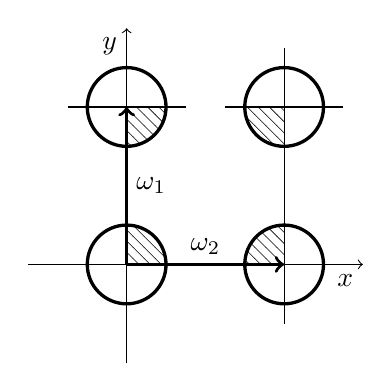
\begin{tikzpicture}[scale=1]
\coordinate (O1) at (0,0);
\coordinate (O2) at (0,2.0);
\coordinate (O3) at (2.0,0);
\coordinate (O4) at (2.0,2.0);

\draw[->] (-1.25,0) -- (3.0,0) node[below left] {$x$};
\draw[->] (0,-1.25) -- (0,3.0) node[below left] {$y$};
\draw[very thick] (O1) circle (0.5);
\draw[very thick] (O2) circle (0.5);
\draw[very thick] (O3) circle (0.5);
\draw[very thick] (O4) circle (0.5);
\draw[very thick, ->] (O1) -- (O2);
\draw[very thick, ->] (O1) -- (O3);
\draw (-0.75,2.0) -- (0.75,2.0);
\draw (2.0,-0.75) -- (2.0,0.75);
\draw (1.25,2.0) -- (2.75,2.0);
\draw (2.0,1.25) -- (2.0,2.75);
\draw (O3) -- (O4);
\filldraw[pattern=custom north west lines,hatchspread=4pt,hatchthickness=0.2pt,hatchcolor=black]
(0,0) -- (0.5,0) arc (0:90:0.5);
\filldraw[pattern=custom north west lines,hatchspread=4pt,hatchthickness=0.2pt,hatchcolor=black]
(2.0,0) -- (1.5,0) arc (180:90:0.5);
\filldraw[pattern=custom north west lines,hatchspread=4pt,hatchthickness=0.2pt,hatchcolor=black]
(2.0,2.0) -- (1.5,2.0) arc (180:270:0.5);
\filldraw[pattern=custom north west lines,hatchspread=4pt,hatchthickness=0.2pt,hatchcolor=black]
(0,2.0) -- (0.5,2.0) arc (360:270:0.5);
\node[right] at (0,1.0) {$\omega_1$}; 
\node[above] at (1.0,0) {$\omega_2$};
%\draw[->] (1.0,0) arc (0:45:1.0);
%\node at (1.1,0.5) {$\alpha$};
\end{tikzpicture}
\end{document}

%%% Local Variables: 
%%% mode: latex
%%% TeX-master: t
%%% End: 
